\documentclass{article}

\usepackage{graphicx}
\usepackage{tikz}
\usepackage{tikzsymbols}
\usetikzlibrary{calc,patterns,shapes.geometric}
\pagestyle{empty}
\usepackage[margin=0pt]{geometry}
\geometry{papersize={14in,12in}}

\def\centerarc[#1](#2)(#3:#4:#5){\draw[#1] ($(#2)+({#5*cos(#3)},{#5*sin(#3)})$) arc (#3:#4:#5);}

\begin{document}
	\begin{figure}
		\centering
		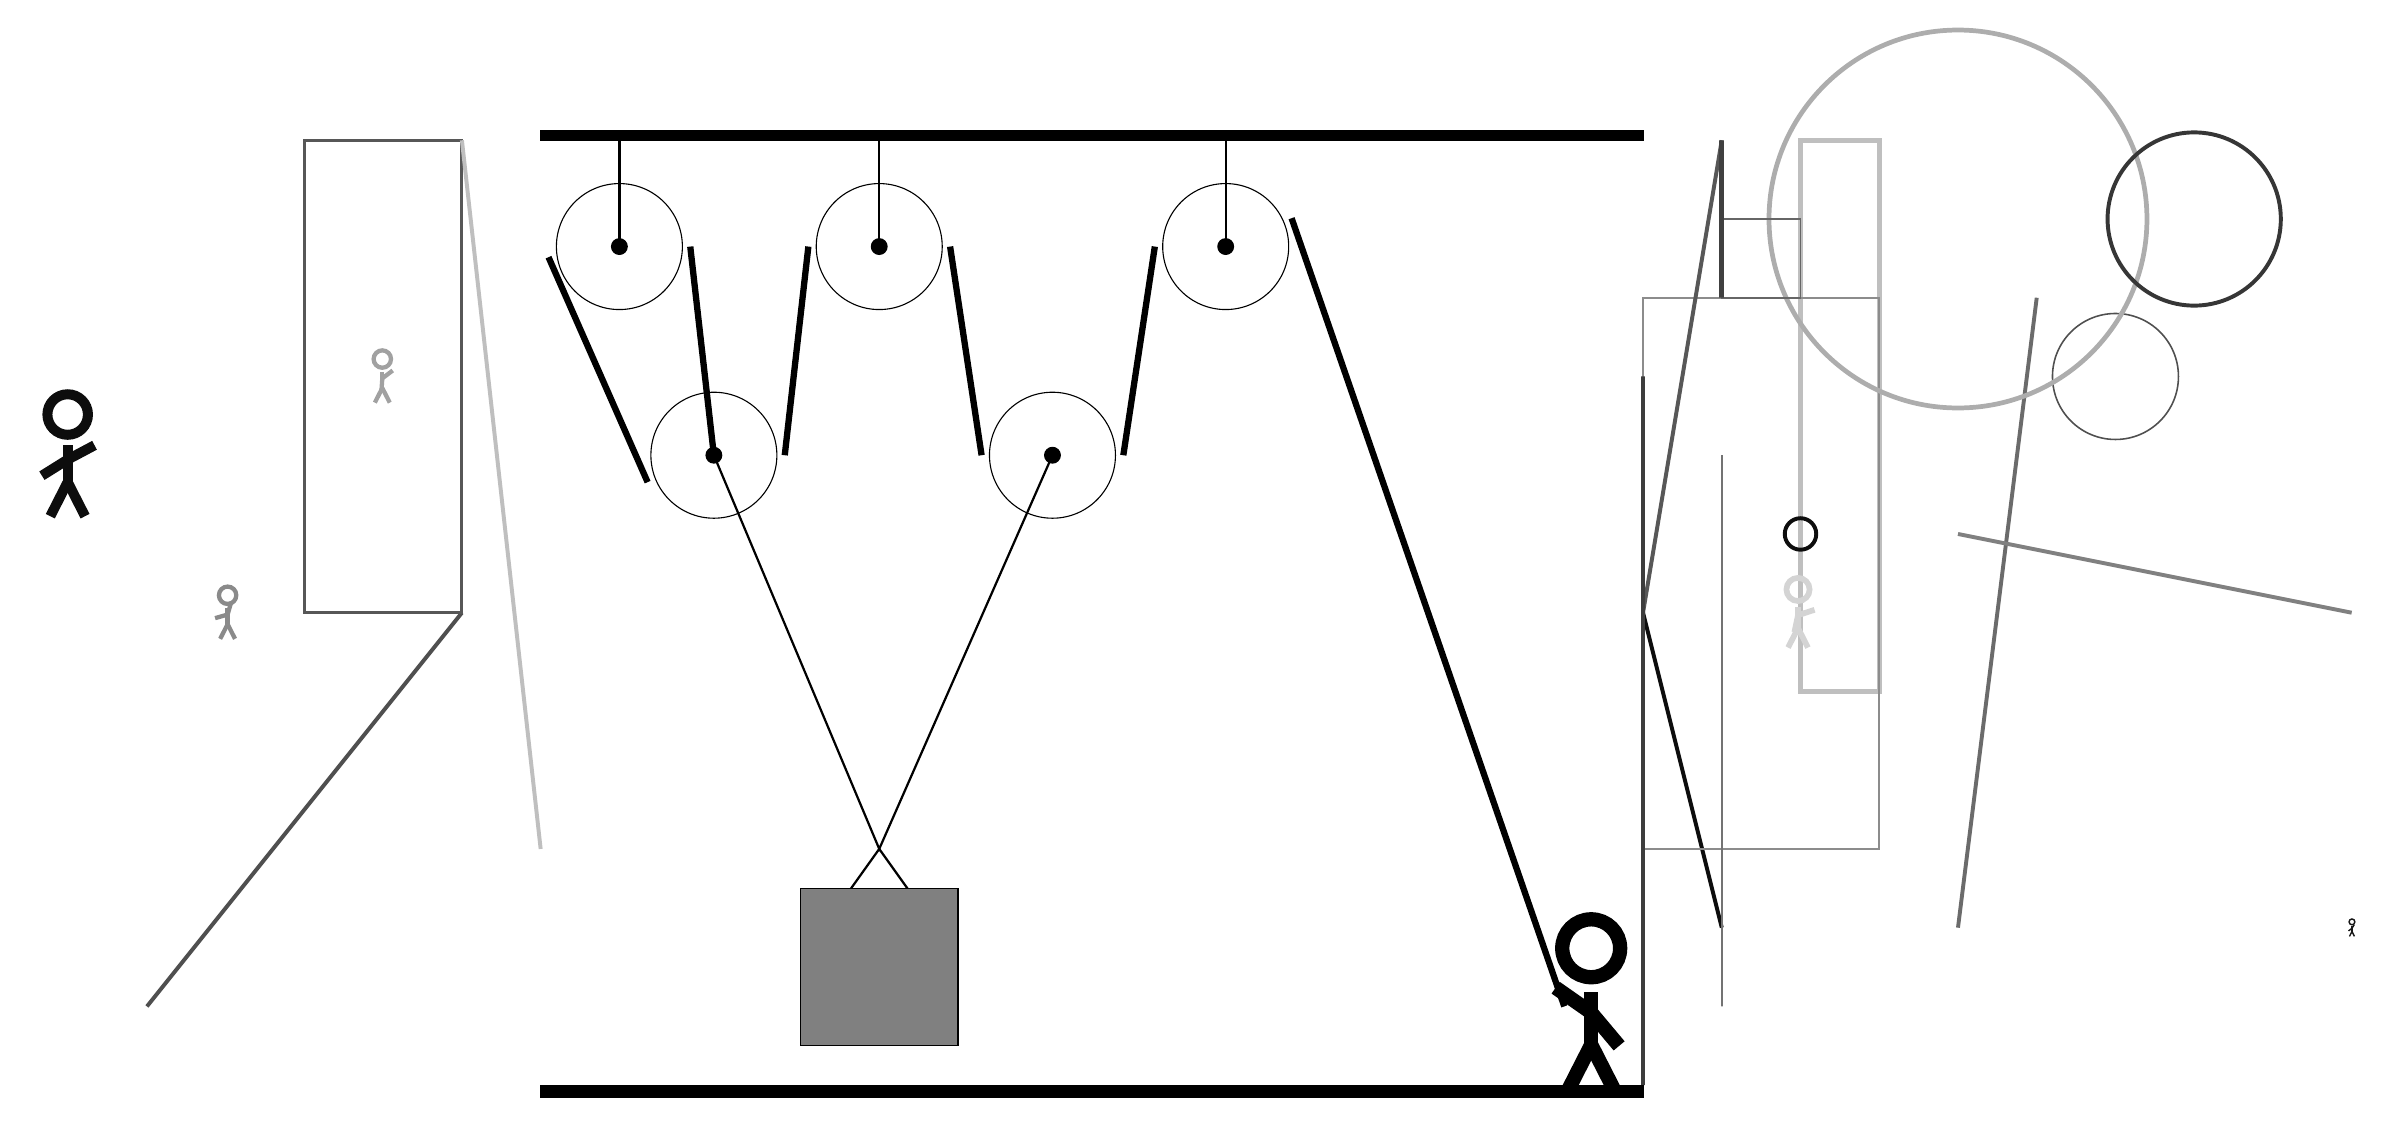
\begin{tikzpicture}
			%%%%% START %%%%%
			
			\draw[fill=black] (-2, 9) rectangle (12, 9.125);
			
			\draw[line width=0.5mm, color=black!58](17, 7) -- (16, -1);
			
			\draw[line width=0.5mm, color=black!69](-7, -2) -- (-3, 3);
			\draw[line width=0.6mm, color=black!25] (14, 9) rectangle (15, 2);
			\node[line width=0.7mm, color=black!17] at (14, 3) {\Strichmaxerl[4][78][18]};
			\draw[line width=0.4mm, color=black!66] (-3, 3) rectangle (-5, 9);
			\node[line width=0.2mm, color=black!46] at (-6, 3) {\Strichmaxerl[3][16][74]};
			\node[line width=0.2mm, color=black!95] at (-8, 5) {\Strichmaxerl[7][32][28]};
			
			\draw[line width=0.5mm, color=black!25](-2, 0) -- (-3, 9);
			\draw[line width=0.5mm, color=black!95](12, 3) -- (13, -1);
			
			\draw [line width=0.2mm, color=black!69](18, 6) circle (0.8);
			\draw[line width=0.2mm, color=black!45] (12, 0) rectangle (15, 7);
			
			\draw [line width=0.6mm, color=black!32](16, 8) circle (2.4);
			\draw[line width=0.5mm, color=black!66](12, 3) -- (13, 9);
			
			\draw[line width=0.2mm, color=black!60] (14, 8) rectangle (13, 7);
			\node[line width=0.7mm, color=black!91] at (21, -1) {\Strichmaxerl[1][37][58]};
			\draw [line width=0.5mm, color=black!79](19, 8) circle (1.1);
			
			\draw[line width=0.2mm, color=black!55] (13, -2) rectangle (13, 5);
			
			\draw[line width=0.5mm, color=black!50](16, 4) -- (21, 3);
			\draw[line width=0.5mm, color=black!76] (12, 6) rectangle (12, -3);
			
			\node[line width=0.5mm, color=black!37] at (-4, 6) {\Strichmaxerl[3][86][37]};
			\draw[line width=0.6mm, color=black!75] (13, 7) rectangle (13, 9);
			
			\draw [line width=0.5mm, color=black!95](14, 4) circle (0.2);
			
			
			\draw (-1, 7.65) circle (0.8);
			\draw[fill=black] (-1, 7.65) circle (0.1);
			\draw[thick] (-1, 7.65) -- (-1, 9);
			
			\draw (2.3, 7.65) circle (0.8);
			\draw[fill=black] (2.3, 7.65) circle (0.1);
			\draw[thick] (2.3, 7.65) -- (2.3, 9);
			
			\draw (6.7, 7.65) circle (0.8);
			\draw[fill=black] (6.7, 7.65) circle (0.1);
			\draw[thick] (6.7, 7.65) -- (6.7, 9);
			
			\draw (0.2, 5) circle (0.8);
			\draw[fill=black] (0.2, 5) circle (0.1);
			
			\draw (4.5, 5) circle (0.8);
			\draw[fill=black] (4.5, 5) circle (0.1);
			
			\draw[thick] (0.2, 5) -- (2.3, 0)  -- (4.5, 5);
			\draw[thick]  (1.8, -0.7) -- (2.3, 0) -- (2.8, -0.7);
			\draw[fill=black!50] (1.3, -0.5) rectangle (3.3, -2.5);
			
			\draw[line width=0.8mm] (0.2, 5) -- (-0.1, 7.65);
			\centerarc[line width=0.8mm](-1, 7.65)(0:200:0.9);
			\draw[line width=0.8mm] (-1.9, 7.515) -- (-0.6415, 4.658);
			\centerarc[line width=0.8mm](0.2, 5)(200:360:0.9);
			\draw[line width=0.8mm](1.1, 5) -- (1.4, 7.65);
			\centerarc[line width=0.8mm](2.3, 7.65)(0:180:0.9);
			\draw[line width=0.8mm] (3.2, 7.65) -- (3.6, 5);
			\centerarc[line width=0.8mm](4.5, 5)(180:360:0.9);
			\draw[line width=0.8mm] (5.4, 5) -- (5.8, 7.65);
			\centerarc[line width=0.8mm](6.7, 7.65)(20:180:0.9);
			\draw[line width=0.8mm](7.537, 8.01)  -- (11, -2);
			
			\node at (11.3, -2) {\Strichmaxerl[10][-35][-50]};
			
			\draw[fill=black] (-2, -3) rectangle (12, -3.15);
			
			%%%%% END %%%%%
		\end{tikzpicture}
	\end{figure}	
\end{document}